\documentclass{beamer}
\usepackage[T1]{fontenc}
\usepackage[utf8]{inputenc}
\usepackage{float}




\title{\textbf{Caratterizzazione e Clustering di Matrici di Correlazione ADNI-2 Tramite Distribuzione di Wishart }}
\author{Carlo Mengucci}
\date{28 Novembre 2017}
\institute{ALMA MATER STUDIORUM $\cdot$ UNIVERSIT\'A DI BOLOGNA}

\usetheme{CambridgeUS}
\setbeamertemplate{blocks}[rounded][shadow=true]

\begin{document}

\begin{frame}
\maketitle
\end{frame}

\begin{frame}
\begin {columns}
\begin{column}{0.8\linewidth}
\begin{block}{Obiettivi dello Studio}

\begin{itemize}
\item Organizzazione ed esplorazione preliminare della sezione del DataBase ADNI-2 contenente le matrici di correlazione di \textit{Resting State} di soggetti sani e affetti da Alzheimer

\item Giustificazione analitica dell'utilizzo della \textit{Distribuzione di Wishart} come ipotesi nulla per la caratterizzazione 

\item Sviluppo di un algoritmo in grado di separare i soggetti sani dai malati e di individuare un gruppo di significativo di \textit{features}  per il clustering
\end{itemize}

\end{block}


\end{column}
\end{columns}
\end{frame}	

\section{Data Structure}

\begin{frame}
\begin {columns}
\begin{column}{0.8\linewidth}
\begin{block}{ADNI-2}

\begin{itemize}
\item 404 soggetti totali

\item Ad ogni soggetto è associata una matrice di correlazione $N\times N$, $N=549$

\item Ognuno degli N elementi rappresenta un \textit{Macrovoxel} di cui è estratta la correlazione \textit{topologica} rispetto a tutte le altre componenti del sistema

\item Ogni \textit{Macrovoxel} è definito su un insieme di $3\cdot10^3$ Voxel

\item Dei 404 soggetti sono stati utilizzati soltanto gli ultimi 300 a causa di discrepanze tra procedure di normalizzazione tra due sezioni distinte individuabili all'interno del  DataBase

\end{itemize}


\end{block}


\end{column}
\end{columns}
\end{frame}

\section{Distribuzione di Wishart}

\begin{frame}
\begin {columns}
\begin{column}{0.8\linewidth}
\begin{block}{Forma Analitica \footnote{\textit{Hardle, Wolfgang and Leopold Simar. 2012. Applied Multivariate Statistical Analysis. Heidelberg: Springer Berlin Heidelberg}}}

\begin{itemize}
\item La distribuzione di Wishart consiste in una famiglia di distribuzioni per \textit{matrici simmetriche definite positive}

\item Siano $X_1...X_n$ vettori indipendenti $N_p(0,\Sigma)$ e tali da formare una matrice di dati $p\times n$, $X=[X_1...X_n]$.
La distribuzione di \textit{matrici random} $p\times p$, $M=XX'=\Sigma^n_{i=1}X_iX_i'$ è una distribuzione di Wishart.
\end{itemize}


\end{block}


\end{column}
\end{columns}
\end{frame}

\begin{frame}
\begin {columns}
\begin{column}{0.8\linewidth}
\begin{block}{Forma Analitica \footnote{\textit{Hardle, Wolfgang and Leopold Simar. 2012. Applied Multivariate Statistical Analysis. Heidelberg: Springer Berlin Heidelberg}}}

\begin{itemize}
\item La matrice random $M_{p\times p}=\Sigma^n_{i=1}X_iX_i'$ segue una distribuzione di Wishart a $n$ gradi di libertà e \textit{matrice di covarianza} $\Sigma$ ed è definita $M\sim W_p(n, \Sigma)$.
Per $n\geq p$ la \textit{pdf} di $M$ assume la forma :
\begin{equation}
f(M)=\frac{1}{2^{\frac{np}{2}}\Gamma_p(\frac{n}{2})\|\Sigma\|^{\frac{n}{2}}}\|M\|^{\frac{n-p-1}{2}}exp[-\frac{1}{2}trace(\Sigma^{-1}M)]
\end{equation}

\item La Wishart può essere interpretata come l'estensione multivariata di una distribuzione $\chi^2$

\end{itemize}

\end{block}


\end{column}
\end{columns}
\end{frame}


\begin{frame}
\begin {columns}
\begin{column}{0.8\linewidth}
\begin{block} {Definizione delle Condizioni di Applicazione}
\begin{itemize}
\item Le matrici di correlazione sono per definizione simmetriche definite positive

\item Il numero $n$ di gradi di libertà del sistema è dato dal campionamento $(n=3\cdot 10^3)$ del singolo Macrovoxel

\item Utilizzando come matrice di scala la matrice data dalla media delle matrici di correlazione delle due categorie di soggetti, è possibile ricostruire la Wishart attesa per le categorie stesse.

\end{itemize}

\end{block}


\end{column}
\end{columns}
\end{frame}

\section{Algoritmo e Clustering}


\begin{frame}
\begin {columns}
\begin{column}{0.8\linewidth}
\begin{block} {Pipeline}

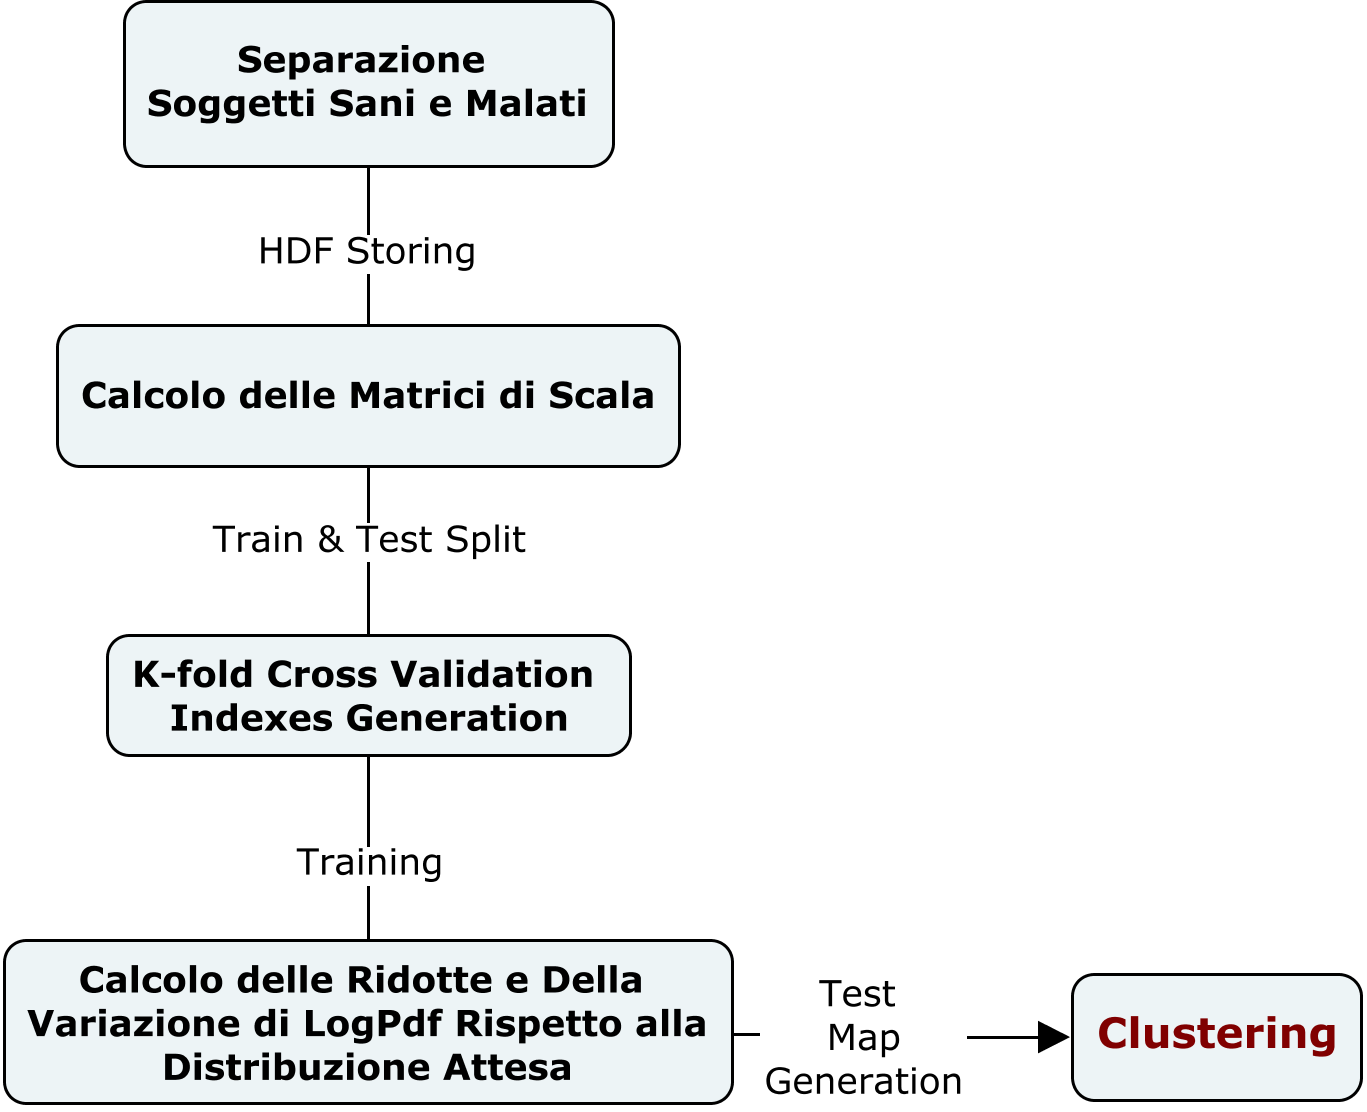
\includegraphics[scale=0.2]{ADNI-alg}


\end{block}


\end{column}
\end{columns}
\end{frame}


\begin{frame}
\begin {columns}
\begin{column}{0.8\linewidth}
\begin{block} {Calcolo delle Ridotte: Approfondimento}

\begin{itemize}
\item \textit{Definizione}: sia $A$ una matrice $n \times n$, una sottomatrice $k \times k$ di $A$ ottenuta eliminando $n-k$ righe e le stesse $n-k$ colonne di $A$ è detta \textit{sottomatrice principale}.

\item \textit{Teorema}: Se $A$ è simmetrica definita positiva, ogni sottomatrice principale di $A$ è anch'essa simmetrica definita positiva.

\item Queste proprietà permettono di calcolare il peso che ogni componente del sistema possiede, in termini di variazione di LogPdf rispetto alla matrice di scala generatrice della distribuzione attesa.

\item Vengono cioè valutate $N$ variazioni di LogPdf su $N$ sottomatrici principali di dimensioni $(N-1) \times (N-1)$.

\end{itemize}

\end{block}

\end{column}
\end{columns}
\end{frame}


\begin{frame}
\begin {columns}
\begin{column}{0.8\linewidth}
\begin{block}{Clustering}
\centering
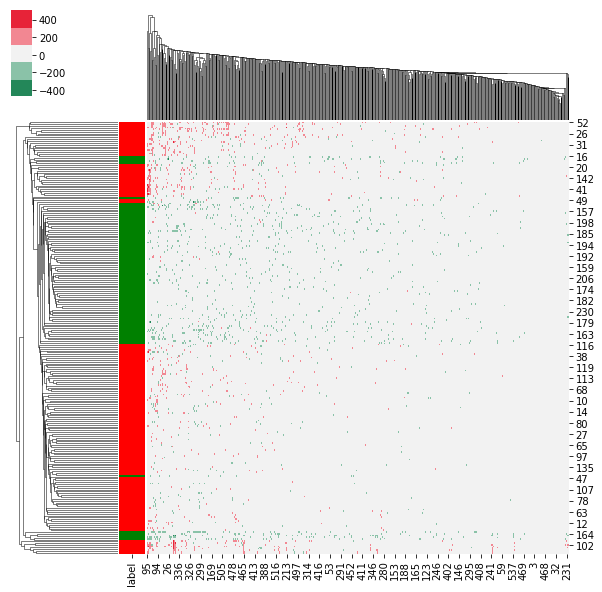
\includegraphics[scale=0.38]{diff-logpdf-clustering10}

\end{block}


\end{column}
\end{columns}
\end{frame}

\begin{frame}
\begin {columns}
\begin{column}{0.8\linewidth}
\begin{block}{LogPdf Distribution}
\centering
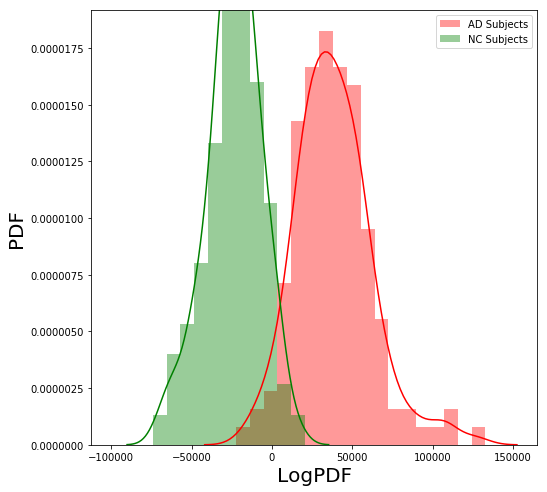
\includegraphics[scale=0.45]{logpdf-dist}

\end{block}


\end{column}
\end{columns}
\end{frame}


\end{document}


